\chapter{Abbildungen, Tabellen, Quellcode}
\label{cha:Abbildungen}

\section{Allgemeines}

Abbildungen (\emph{figures}) und Tabellen (\emph{tables}) werden
üblicherweise zusammen mit einem nummerierten Titel (\emph{caption})
zentriert angeordnet (siehe Abb.~\ref{fig:CocaCola}). Im Text \emph{muss} es
zu jeder Abbildung einen Verweis geben und die eigentliche Abbildung sollte
im \latex-Quelltext erst \emph{nach} dem ersten Verweis platziert werden.

\begin{figure}
	\centering
	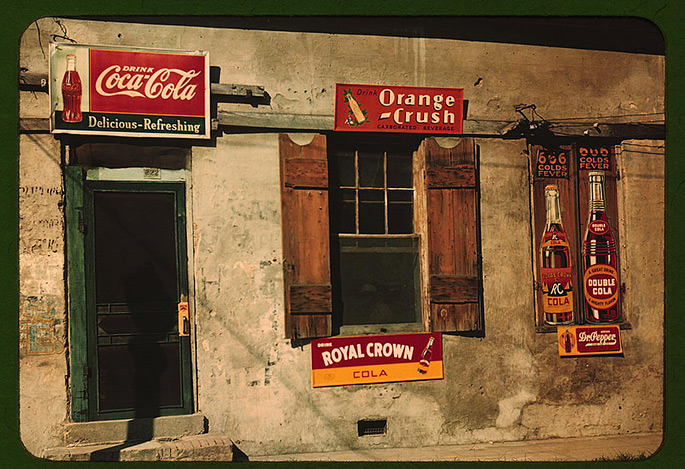
\includegraphics[width=.75\textwidth]{cola-public-domain-photo-p} %{CS0031}
	\caption{Coca-Cola Werbung 1940 \cite{CocaCola1940}.}
	\label{fig:CocaCola}
\end{figure}


\section{\emph{Let Them Float!}}

Das Platzieren von Abbildungen und Tabellen gehört zu den schwierigsten
Aufgaben im Schriftsatz, weil diese meist viel Platz benötigen und häufig
nicht auf der aktuellen Seite im laufenden Text untergebracht werden können.
Diese Elemente müssen daher an eine geeignete Stelle auf nachfolgenden Seiten
verschoben werden, was manuell sehr mühsam (jedoch in \emph{Word}
beispielsweise unerlässlich) ist.

In \latex funktioniert das weitgehend automatisch, indem Abbildungen,
Tabellen und ähnliche als "Floating Bodies" behandelt werden. Bei der
Positionierung dieser Elemente wird versucht, einerseits im Textfluss
möglichst wenig Leer\-raum entstehen zu lassen und andererseits die
Abbildungen und Tabellen nicht zu weit von der ursprünglichen Textstelle zu
entfernen.

Der Gedanke, dass etwa Abbildungen kaum jemals genau an der ge\-wünsch\-ten
Stelle und möglicherweise nicht einmal auf derselben Seite Platz finden, ist
für viele Anfänger*innen aber offenbar sehr ungewohnt oder sogar beängstigend.
Dennoch sollte zunächst einmal getrost \latex\ diese Arbeit überlassen und
\emph{nicht} manuell eingegriffen werden. Erst am Ende, wenn das gesamte
Dokument "steht" und die automatische Platzierung wirklich nicht
zufriedenstellend erscheint, sollte (durch gezielte Platzierungsanweisungen
\cite[S.~39]{Oetiker2021}) \textbf{in Einzelfällen} eingegriffen werden.


\section{Captions}

Bei Abbildungen steht der Titel üblicherweise \emph{unten}, bei Tabellen
hingegen -- je nach Konvention -- \emph{oben} (wie in diesem Dokument) oder
ebenfalls \emph{unten}. In \latex\ erfolgt auch die Nummerierung der
Abbildungen automatisch, ebenso der Eintrag in das (optionale)
Abbildungsverzeichnis%
\footnote{Ein eigenes Verzeichnis der Abbildungen am Ende des Dokuments ist
zwar leicht erstellt, in einer Abschlussarbeit aber (und eigentlich überall
sonst auch) überflüssig. Man sollte es daher weglassen. Sollte der*die
Betreuer*in dennoch darauf bestehen, findet sich im Wiki des
\texttt{hagenberg-thesis} GitHub-Repositorys eine Anleitung zur Integration ins
eigene Dokument.} am Ende des Dokuments.

Die Markierung der Captions%
\footnote{Ausnahmsweise wird das Wort "Caption" im Folgenden ohne deutsche
	Übersetzung verwendet.}
erfolgt in \latex mithilfe der \verb!\label{}! Anweisung, die unmittelbar auf
die \verb!\caption{}! Anweisung folgen muss:
%
\begin{LaTeXCode}[numbers=none]
\begin{figure}
	\centering
	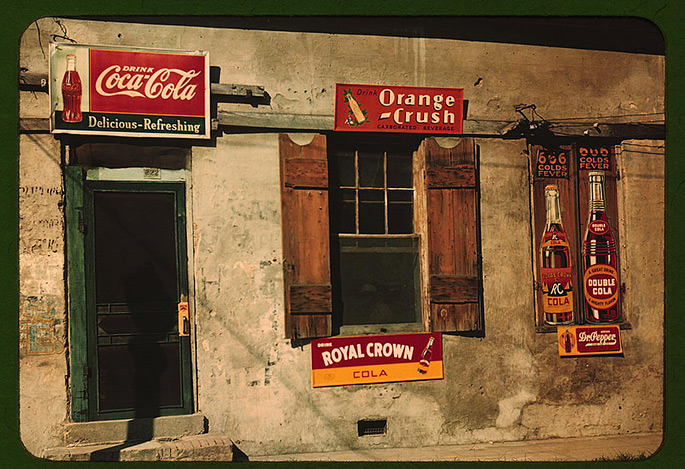
\includegraphics[width=.95\textwidth]{cola-public-domain-photo-p}
	\caption{Coca-Cola Werbung 1940 \cite{CocaCola1940}.}
	\label{fig:CocaCola}
\end{figure}
\end{LaTeXCode}
%
Der Name des Labels (\texttt{fig:CocaCola}) kann beliebig gewählt werden. Die
Kennzeichnung \texttt{fig:} ist (wie in Abschn.\ \ref{sec:querverweise}
erwähnt) nur eine nützliche Hilfe, um beim Schreiben verschiedene Arten von
Labels besser unterscheiden zu können.

Die Länge der Captions kann dabei sehr unterschiedlich sein. Je nach
Anwendung und Stil ergibt sich manchmal eine sehr kurze Caption
(Abb .~\ref{fig:CocaCola}) oder eine längere (Abb.~\ref{fig:ibm360}).
Man beachte, wie bei kurzen Captions ein zentrierter Satz und bei langen
Captions ein Blocksatz verwendet wird (\latex macht das automatisch).
Captions sollten \emph{immer} mit einem Punkt abgeschlossen sein.%
\footnote{Kurioserweise verlangen manche Anleitungen genau das Gegenteil,
	angeblich, weil beim klassischen Bleisatz die abschließenden Punkte im
	Druck häufig "weggebrochen" sind. Das kann man glauben oder nicht, im
	Digitaldruck spielt es jedenfalls keine Rolle.}

\begin{figure}
	\centering
	\fbox{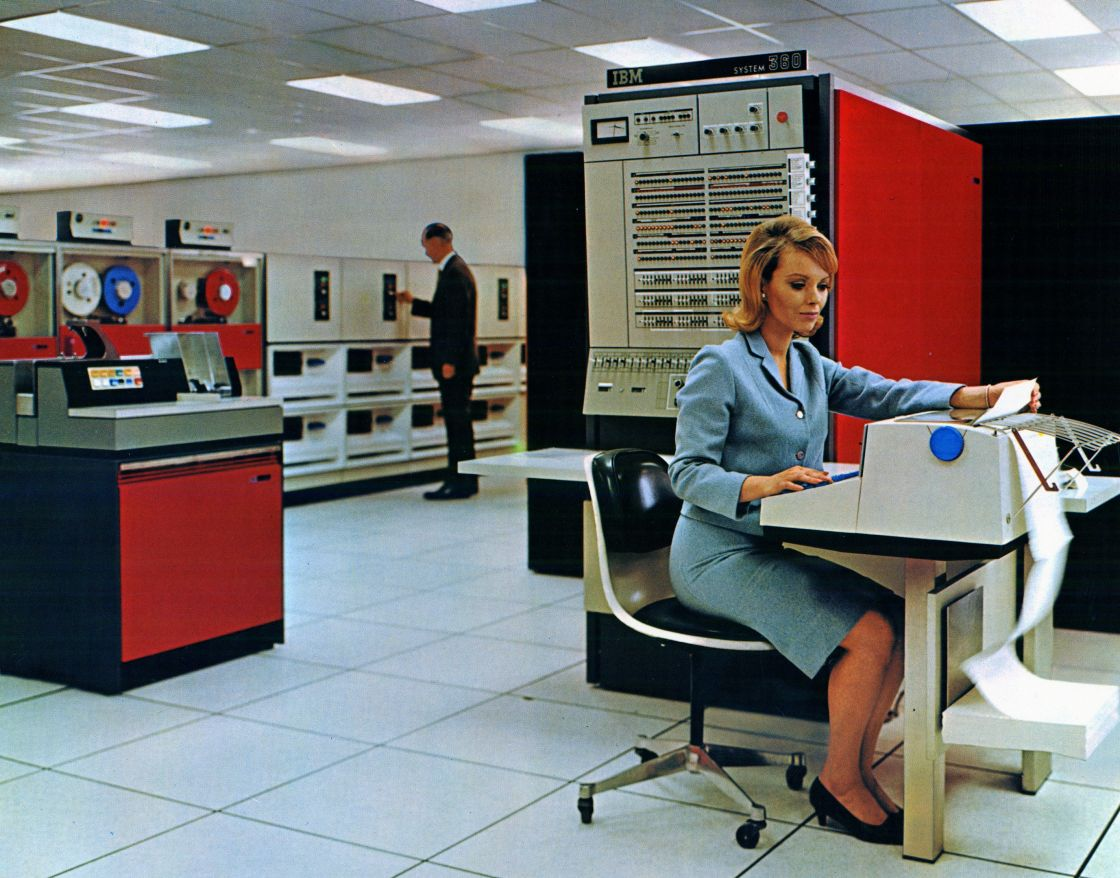
\includegraphics[width=.75\textwidth]{ibm-360-color}}
	\caption{Beispiel für einen langen Caption-Text. \textsc{Univac} brachte
	1961 mit dem Modell 751 den ersten Hochleistungsrechner mit
	Halbleiterspeicher auf den Markt. Von diesem Computer wurden in den U.S.A.\
	bereits im ersten Produktionsjahr über fünfzig Exemplare verkauft,
	vorwiegend an militärische Dienststellen, Versicherungen und
	Großbanken. Die Ablöse erfolgte zwei Jahre später durch das zusammen
	mit \textsc{Sperry} entwickelte Modell 820. Das klingt vielleicht
	plausibel, ist aber völliger Unsinn, und das Bild zeigt in Wirklichkeit
	eine System/360 Anlage von IBM. Bildquelle~\cite{IBM360}.}
	\label{fig:ibm360}
\end{figure}


\section{Abbildungen}

Für die Einbindung von Grafiken in \latex wird die Verwendung des
Stan\-dard-Pakets \texttt{graphicx} \cite{Carlisle2021} empfohlen (wird durch
das \texttt{hagenberg-thesis}-Paket bereits eingebunden). Mit dem aktuell
verwendeten Workflow (\texttt{pdflatex}) können Bild- bzw.\ Grafikformate
ausschließlich in folgenden Formaten eingebunden werden:
%
\begin{itemize}
	\item \textbf{PNG}: für Grau-, S/W- und Farb-Rasterbilder (bevorzugt),
	\item \textbf{JPEG}: für Fotos (wenn nicht anders vorhanden),
	\item \textbf{PDF}: für Vektorgrafiken (Illustrationen, Strichzeichnungen \etc).
\end{itemize}
%
Bei Rasterbildern sollte wenn möglich PNG verwendet werden, weil die darin
enthaltenen Bilder verlustfrei komprimiert sind und daher keine sichtbaren
Kompressionsartefakte aufweisen. Im Gegensatz dazu sollte JPEG nur dann
verwendet werden, wenn das Originalmaterial (Foto) bereits in dieser Form
vorliegt.


\subsection{Wo liegen die Grafikdateien?}

Die Bilder werden üblicherweise in einem Unterverzeichnis (oder in mehreren
Unterverzeichnissen) abgelegt, im Fall dieses Dokuments in
\nolinkurl{images/}. Dazu dient die folgende Anweisung am Beginn des
Hauptdokuments \nolinkurl{main.tex} (\sa\ Anhang \ref{app:latex}):
%
\begin{quote}
	\verb!\graphicspath{{images/}}!
\end{quote}
%
Der (zum Hauptdokument relative) Pfad \texttt{graphicspath} kann innerhalb
des Dokuments jederzeit geändert werden, was durchaus nützlich ist, wenn \zB\
die Grafiken einzelner Kapitel getrennt in entsprechenden Verzeichnissen
abgelegt werden sollen.
Die Größe der Abbildung im Druck kann durch Vorgabe einer bestimmten Breite
oder Höhe oder eines Skalierungsfaktors gesteuert werden, {\zB}:
%
\begin{quote}
	\verb!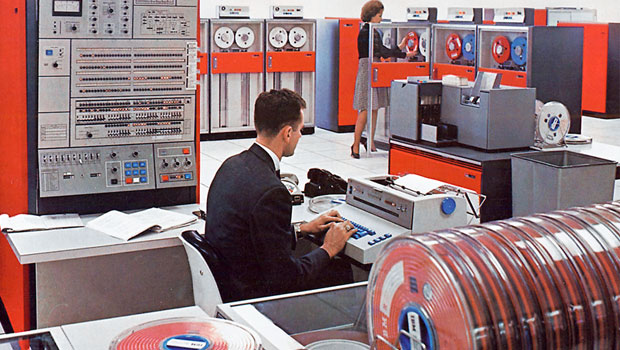
\includegraphics[width=.85\textwidth]{ibm-360-color}! \\
	\verb!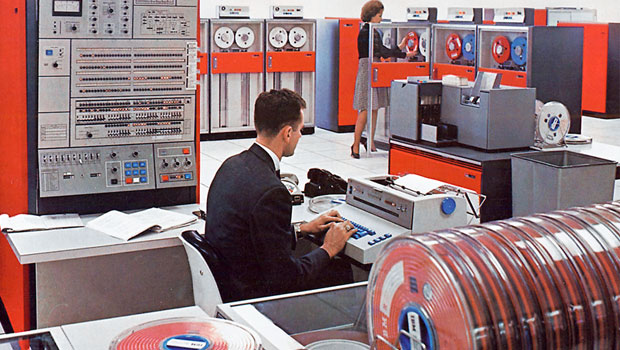
\includegraphics[scale=1.5]{ibm-360-color}!
\end{quote}
%
Man beachte, dass dabei die Dateiendung nicht explizit angegeben werden muss.
Das ist \va\ dann praktisch, wenn verschiedene Workflows mit jeweils
unterschiedlichen Dateitypen verwendet werden.


\subsection{Grafiken einrahmen}

Mit dem Makro \verb!\fbox{...}! kann optional ein dünner Rahmen rund um die
Grafik erzeugt werden, \zB:
%
\begin{quote}
	\verb!\fbox{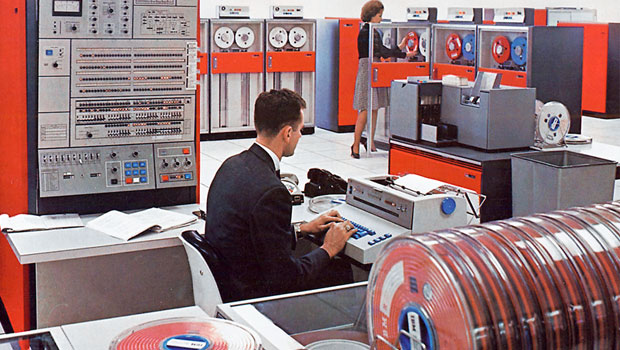
\includegraphics[height=50mm]{ibm-360-color}}!
\end{quote}
%
Das wird üblicherweise nur bei Rasterbildern nötig sein, insbesondere wenn
sie zum Rand hin sehr hell sind und ohne Rahmen nicht vom Hintergrund
abgrenzbar wären.

\subsection{Rasterbilder (Pixelgrafiken)}

Generell sollten Bilder bereits vorher so aufbereitet werden, dass sie später
beim Druck möglichst wenig an Qualität verlieren. Es empfiehlt sich daher,
die Bildgröße (Auflösung) bereits im Vorhinein (\zB mit \emph{Photoshop})
richtig einzustellen.
Brauchbare Auflösungen bezogen auf die endgültige Bildgröße sind:
%
\begin{itemize}
  \item \textbf{Farb- und Grauwertbilder:} 150--300 dpi,
  \item \textbf{Binärbilder (Schwarz/Weiß):} 300--600 dpi.
\end{itemize}
%
Eine wesentlich höhere Auflösung macht aufgrund der beim Laserdruck
notwendigen Rasterung keinen Sinn, auch bei 1200 dpi-Druckern. Speziell
\emph{Screen\-shots} sollten nicht zu klein dargestellt werden, da sie sonst
schlecht lesbar sind (max.\ 200 dpi, besser 150 dpi). Dabei ist zu bedenken,
dass die Arbeit auch als Kopie in allen Details noch gut lesbar sein sollte.

\subsubsection{JPEG-Problematik}

In der Regel sollten Bilder, die für den Einsatz in Druckdokumenten gedacht
sind, nicht mit verlustbehafteten Kompressionsverfahren abgespeichert werden.
Insbesondere sollte die Verwendung von JPEG möglichst vermieden werden, auch
wenn viele Dateien dadurch wesentlich kleiner werden.
Eine Ausnahme ist, wenn die Originaldaten nur in JPEG vorliegen und für die 
Einbindung nicht bearbeitet oder verkleinert wurden. Ansonsten sollte immer
PNG verwendet werden.

Besonders gerne werden farbige \textbf{Screenshots} der JPEG-Kompression%
\footnote{Das JPEG-Verfahren ist für natürliche Fotos konzipiert und sollte
auch nur dafür verwendet werden.}
unter\-zogen, obwohl deren verheerende Folgen für jede*n Laiin*Laien sichtbar
sein sollten (Abb.~\ref{fig:jpeg-pfusch}).

\begin{figure}
	\centering\small
	\begin{tabular}{@{}cc@{}}
		\fbox{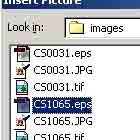
\includegraphics[width=0.475\textwidth]{screenshot-dirty}} &
		% JPEG file
		\fbox{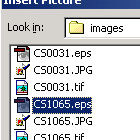
\includegraphics[width=0.475\textwidth]{screenshot-clean}} \\
		% PNG file
		(a) & (b)
	\end{tabular}
	\caption{Typischer JPEG-Pfusch. Screenshots und ähnliche im Original
	verfügbare Rasterbilder sollten für Druckdokumente \emph{keinesfalls} mit
	JPEG komprimiert werden. Das Ergebnis~(a) sieht gegenüber dem
	unkomprimierten Original~(b) nicht nur schmutzig aus, sondern wird
	im Druck auch schnell unleserlich.}
	\label{fig:jpeg-pfusch}
\end{figure}


\subsection{Vektorgrafiken}

Für schematische Abbildungen (\zB Flussdiagramme,
Entity-Relationship-Diagramme oder sonstige strukturelle Darstellungen)
sollten unbedingt Vektorgrafiken (PDF) verwendet werden. Gerasterte Grafiken,
wie sie üblicherweise als GIF- oder PNG-Dateien auf Webseiten vorliegen,
haben in einem Druckdokument nichts zu suchen, notfalls müssen sie mit einem
entsprechenden Werkzeug \emph{neu} gezeichnet werden (natürlich unter Angabe
der ursprünglichen Quelle).

In diesem Fall kommt als Datenformat nur PDF in Frage, dieses bietet sich
aber auch in anderen Umgebungen als universelles Vektor-Format an. Zur
Erstellung von PDF-Vektorgrafiken wird ein geeignetes Grafikprogramm, \zB\
\emph{Adobe Illustrator} oder \emph{Inkscape}, benötigt. Manche gängigen
Grafikprogramme unterstützen allerdings keinen direkten Export von PDF-Dateien
oder erzeugen unsaubere Dateien. Vor der Entscheidung für eine bestimmte
Zeichensoftware sollte das im Zweifelsfall ausprobiert werden. PDF kann im
Notfall über einen entsprechenden Druckertreiber erzeugt werden.


\subsubsection{Einbettung von Schriften}

Die Wiedergabe von Textelementen ist abhängig von der auf dem Computer (oder
Drucker) installierten Schriften und der Form der Schrifteinbettung im
Quelldokument. Die korrekte Darstellung am Bildschirm eines Computers
bedeutet nicht, dass dasselbe Dokument auf einem anderen Computer oder
Drucker genau so dargestellt wird. Dieser Umstand ist besonders wichtig, wenn
Druckdokumente online zur Verfügung gestellt werden. Kontrollieren Sie daher
genau, ob die innerhalb Ihrer Grafiken verwendeten Schriften auch exakt wie
beabsichtigt im Ausdruck aufscheinen 
(\sa\ Abschnitt \ref{sec:tex-schriften-in-grafiken}).


\subsubsection{Strichstärken -- \emph{Hairlines} vermeiden!}

In Grafik-Programmen wie \emph{Illustrator} und \emph{Inkscape}, die sich im
Wesentlichen an der PDF- \bzw\ SVG-Funktionalität orientieren, 
ist es möglich, Linien bzgl.\ ihrer Stärke als "Hairline" zu definieren. Dies 
soll in der Ausgabe "möglichst dünne" Linien erzeugen. Das Ergebnis ist 
aber ausschließlich vom jeweiligen Drucker abhängig und somit kaum 
vorhersagbar. \textbf{Fazit:} Hairlines vermeiden und stattdessen immer 
konkrete Strichstärken ($\geq 0.25\,\mathrm{pt}$) einstellen!


\subsection{\tex-Schriften auch in Grafiken?}
\label{sec:tex-schriften-in-grafiken}

Grundsätzlich sollten auch die in Grafiken verwendete Schriften möglichst genau
mit der Schrift im Haupttext übereinstimmen. Bei Abbildungen, die mit externen
Grafikprogrammen erzeugt werden, kann man
zumindest \emph{ähnlich} aussehende Schriften (wie \emph{Times-Roman} oder
\emph{Garamond}) verwenden. Es ist aber auch möglich, die 
\emph{Computer-Modern} (CM) Schriftfamilie von {\tex}/{\latex} direkt
zur Erzeugung von Grafiken einzusetzen.
Es stehen einige Portierungen von CM als \emph{TrueType}-Schriften zur
Verfügung, die auch in herkömmlichen Grafikprogrammen unter \emph{Windows}
und \emph{Mac~OS} verwendet werden können:
%
\begin{itemize}
\item	%\subsubsection{\emph{BaKoMa}-Schriften (TrueType)}
Empfehlenswert ist \zB\ die "BaKoMa Fonts Collection",%
\footnote{\url{http://ctan.org/pkg/bakoma-fonts}}
die neben den CM Standardschriften auch die mathematischen Schriften der
AMS-Familie ent\-hält und zudem kostenfrei ist. 
\item	%\subsubsection{\emph{Latin Modern Roman} Fonts (OpenType)}
Eine Alternative dazu sind die "LM-Roman"%
\footnote{\url{http://www.gust.org.pl/projects/e-foundry/latin-modern}}
Open-Type Schriften, die speziell für die Verwendung im Umfeld von \latex\
entwickelt wurden. Sie sind auch Teil der MikTeX-Installation.%
\footnote{\zB unter \url{C:/Program Files/MiKTeX 2.9/fonts/opentype/public/lm}}
Diese Schriften enthalten \ua\ Zeichen mit Umlauten und sind daher auch für 
deutsche Texte gut geeignet.
\end{itemize}
%
Natürlich müssen diese Schriften vor der Verwendung zunächst auf dem eigenen PC
installiert werden.

\subsection{Grafiken mit \latex-Overlays (\texttt{overpic})}
\label{sec:GraphicOverlays}

Manchmal ist es erforderlich, ein bestehendes Bilder oder eine Grafik mit
\latex-eigenen (Vektor-){\obnh}Elementen zu überlagern, \zB\ für Markierungen oder
Beschriftungen. Ein typisches Beispiel ist in Abb.~\ref{fig:overpic-example}
gezeigt, wo eine mit \emph{Mathematica} generierte PDF-Grafik mit
mathematischen Elementen annotiert wird.

Dazu wird das \texttt{overpic}-Paket%
\footnote{\url{https://ctan.org/pkg/overpic}}
verwendet, wobei die darunter liegende Grafik nicht mit \verb!\includegraphics!
sondern \verb!\begin{overpic}! \ldots \verb!\end{overpic}! importiert wird
(mit ähnlicher Syntax):

\begin{LaTeXCode}[numbers=none]
\begin{overpic}[width=0.85\textwidth]{mathematica-example}
	\put(101,14){$x$}%
	\put(4,31){$f(x)$}%
	\put(29.5,28){\line(1,1){2}}%
	...
\end{overpic}
\end{LaTeXCode}

\begin{figure}
	\centering\small
	\vspace*{3mm}
	\begin{overpic}[width=0.85\textwidth]{mathematica-example}
		\put(101,14){$x$}%
		\put(4,31){$f(x)$}%
		\put(29.5,28){\line(1,1){2}}%
		{\color{green!70!black}\put(29.5,28){\circle*{2.0}}}%
		\put(32,30){$\cos(\frac{7}{3} x)$}%
		\put(59,28){\line(1,1){2}}%
		{\color{blue!70!black}\put(59,28){\circle*{2.0}}}%
		\put(61.5,30){$\cos(x)$}%
	\end{overpic}
	\caption{Beispiel für die Verwendung des \texttt{overpic}-Pakets zum
	Einfügen von \latex-Elementen über eine importierte Grafik.
	In diesem Fall wurden die mathematischen Elemente $x$, $f(x)$, $\cos(x)$
	und $\smash{\cos(\frac{7}{3} x)}$ sowie zwei diagonale Geraden und
	gefüllte (färbige) Kreise eingefügt. Darunter liegt die Vektor\-grafik
	\texttt{mathematica-example.pdf}.}
	\label{fig:overpic-example}
\end{figure}

Die \texttt{overpic}-Umgebung bildet gleichzeitig eine 
\texttt{picture}-Umgebung,%
\footnote{\url{https://www.overleaf.com/learn/latex/Picture_environment}}
in der \latex-Zeichenanweisungen (wie \verb!\put! u.ä.) platziert werden
können, wie in obigem Beispiel gezeigt.%
\footnote{Die Standard-Zeichenanweisungen in \latex sind ziemlich restriktiv,
weshalb hier zusätzlich das \texttt{pict2e}-Paket 
(\url{https://ctan.org/pkg/pict2e}) verwendet wird.}
Die $x/y$-Positionen sind in Prozent der Bildbreite angegeben. Weitere
Details finden sich im Quelltext.


\subsection{Abbildungen mit mehreren Elementen}

Werden mehrere Bilder oder Grafiken zu einer Abbildung zusammengefasst, wird
üblicherweise eine gemeinsame Caption verwendet, wie in Abb.~\ref{fig:Bearings}
dargestellt. Im Text könnte ein Verweis auf einen einzelnen Teil der
Abbildung, etwa das einreihige Rollenlager in Abb.~\ref{fig:Bearings}\,(c),
so aussehen:
%
\begin{LaTeXCode}[numbers=none]
    ... Abb.~\ref{fig:Bearings} (c) ... 
\end{LaTeXCode}


\subsection{Quellenangaben in Captions}
\label{sec:QuellenangabenInCaptions}

Wenn Bilder, Grafiken oder Tabellen aus anderen Quellen verwendet werden,
dann muss ihre Herkunft in jedem Fall klar ersichtlich gemacht werden, und
zwar am besten direkt in der Caption. Wird beispielsweise eine Grafik aus
einem Buch oder einer sonstigen zitierfähigen Publikation verwendet, dann
sollte diese in das Literaturverzeichnis aufgenommen und wie üblich mit
\verb!\cite{..}! zitiert werden, wie in Abb.\ \ref{fig:Bearings} demonstriert.
Weitere Details zu dieser Art von Quellenangaben finden sich in Kap.\
\ref{cha:Literatur} (insbes.\ Abschnitt \ref{sec:KategorieOnline}).

\begin{figure}
	\centering\small
	\begin{tabular}{@{}c@{\hspace{12mm}}c@{}} % mittlerer Abstand = 12mm
		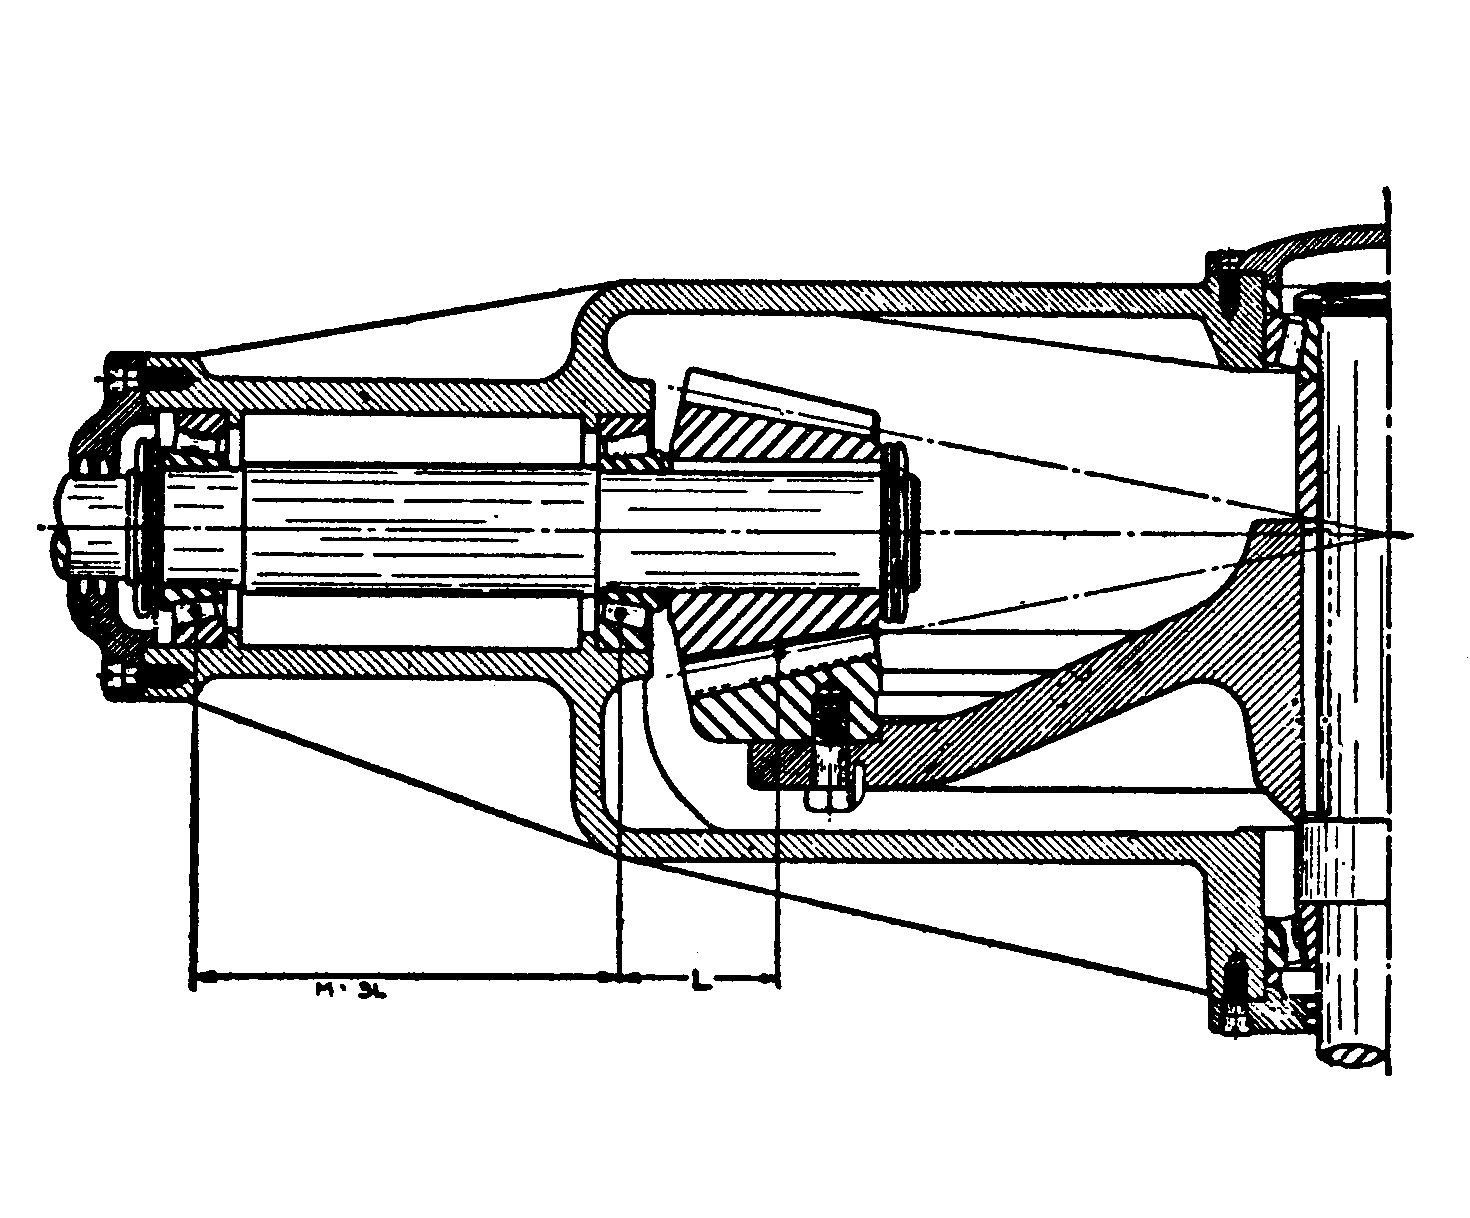
\includegraphics[width=.45\textwidth]{overhang-mounting} &
		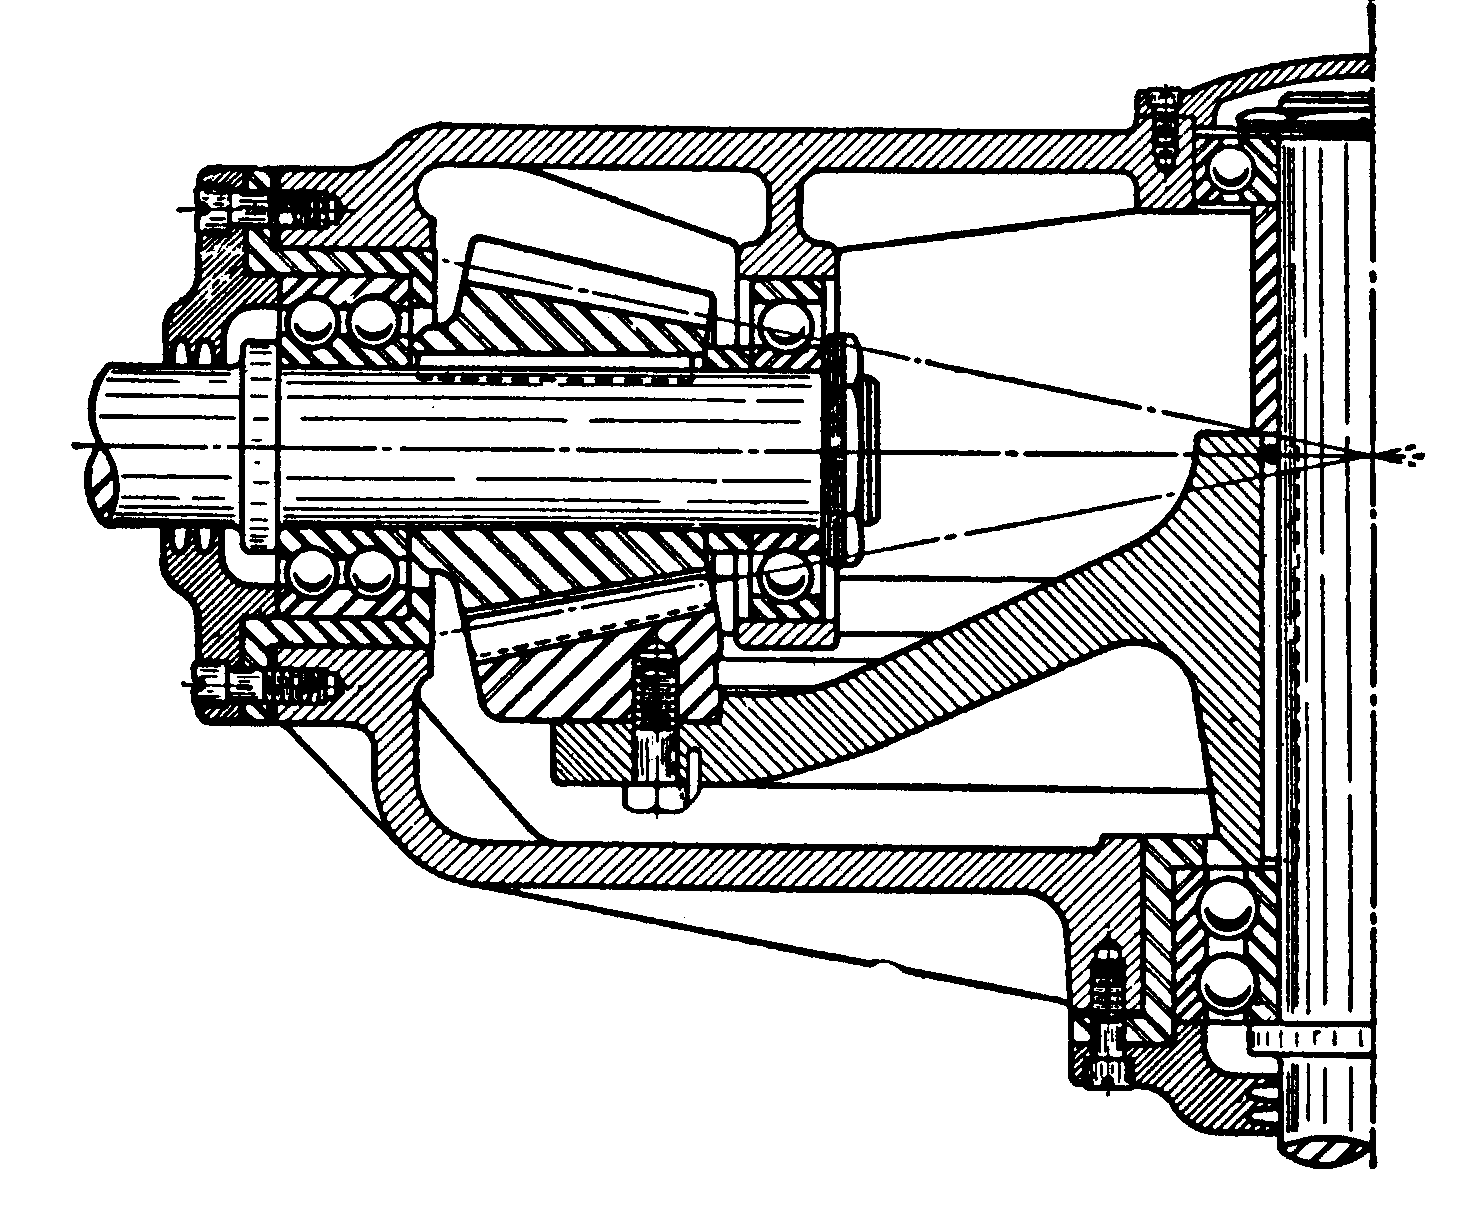
\includegraphics[width=.45\textwidth]{straddle-mounting}
		\\
		(a) & (b)
		\\[4pt]    %vertical extra spacing (4 points)
		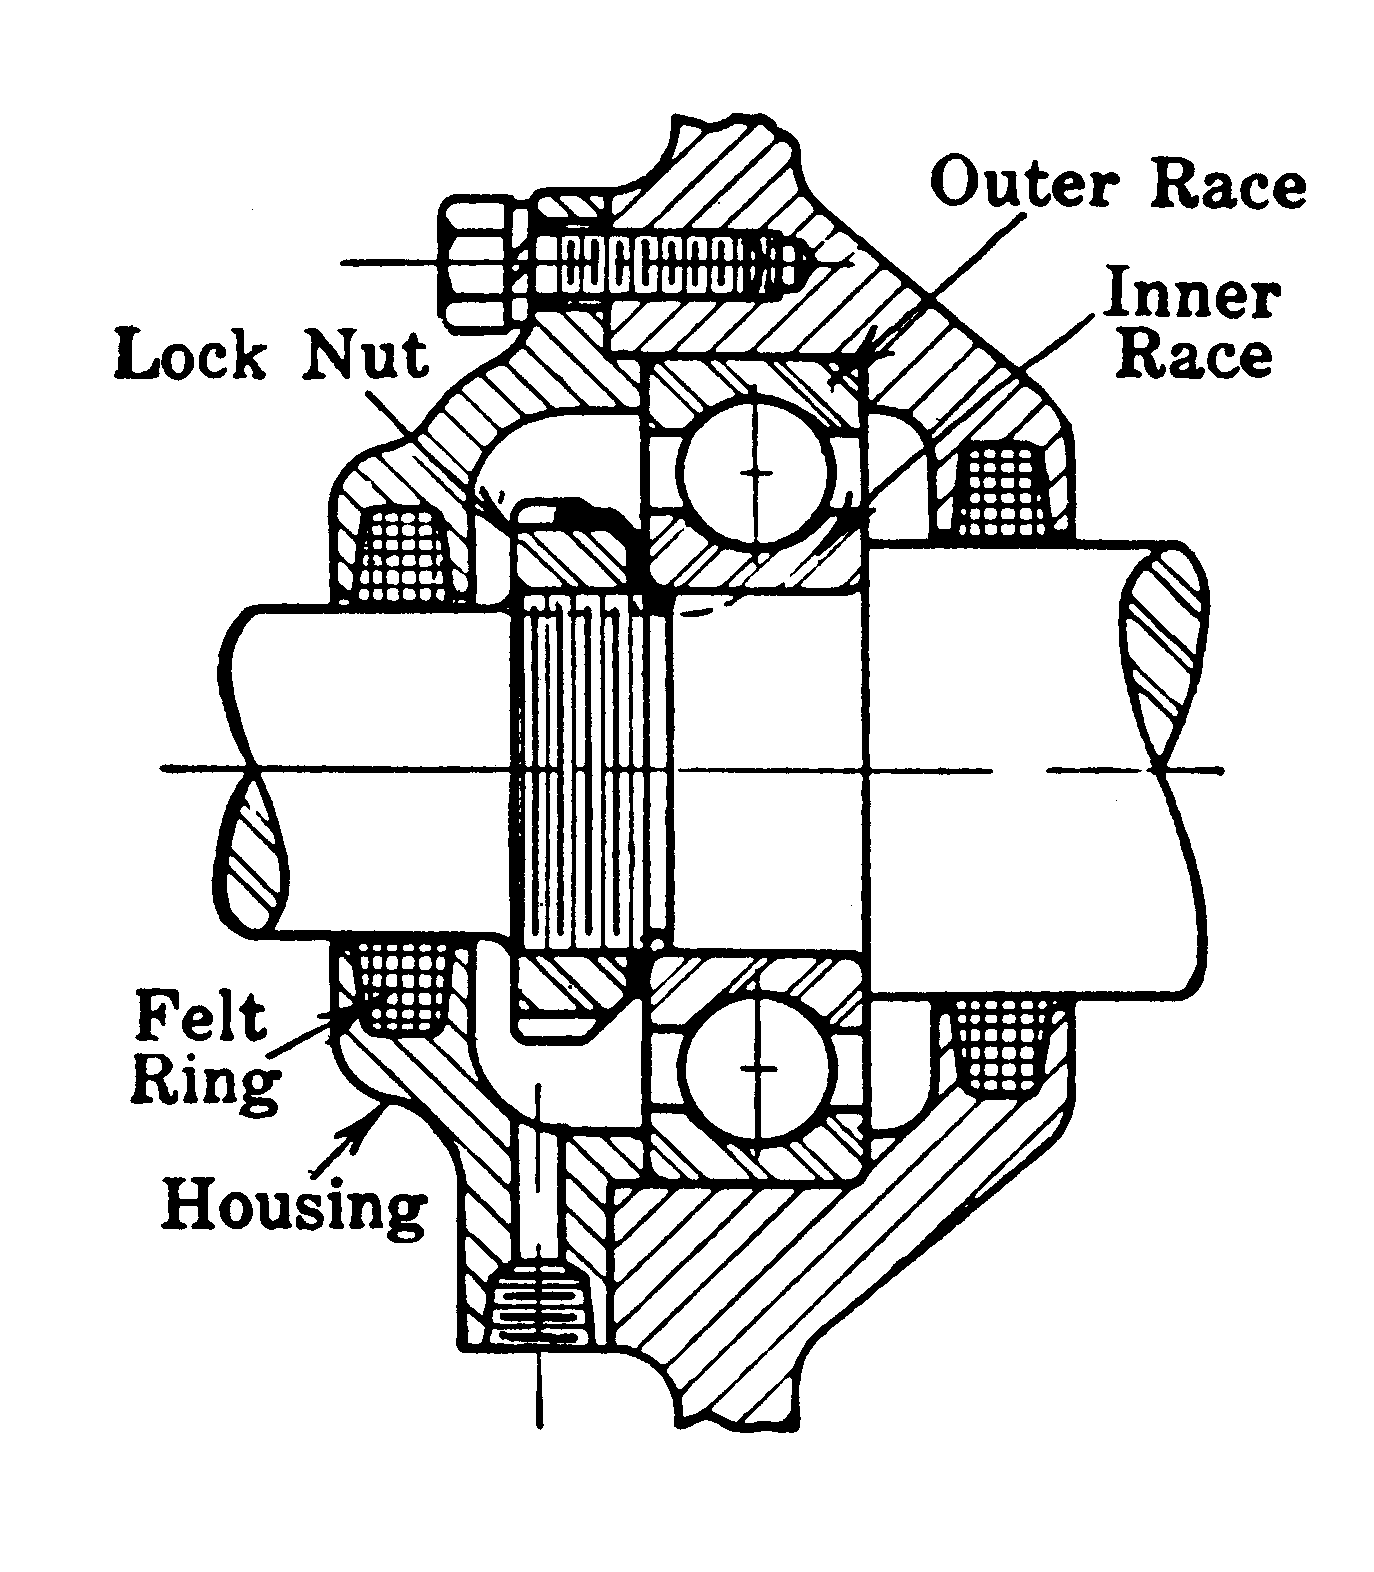
\includegraphics[width=.45\textwidth]{ball-bearing-1} &
		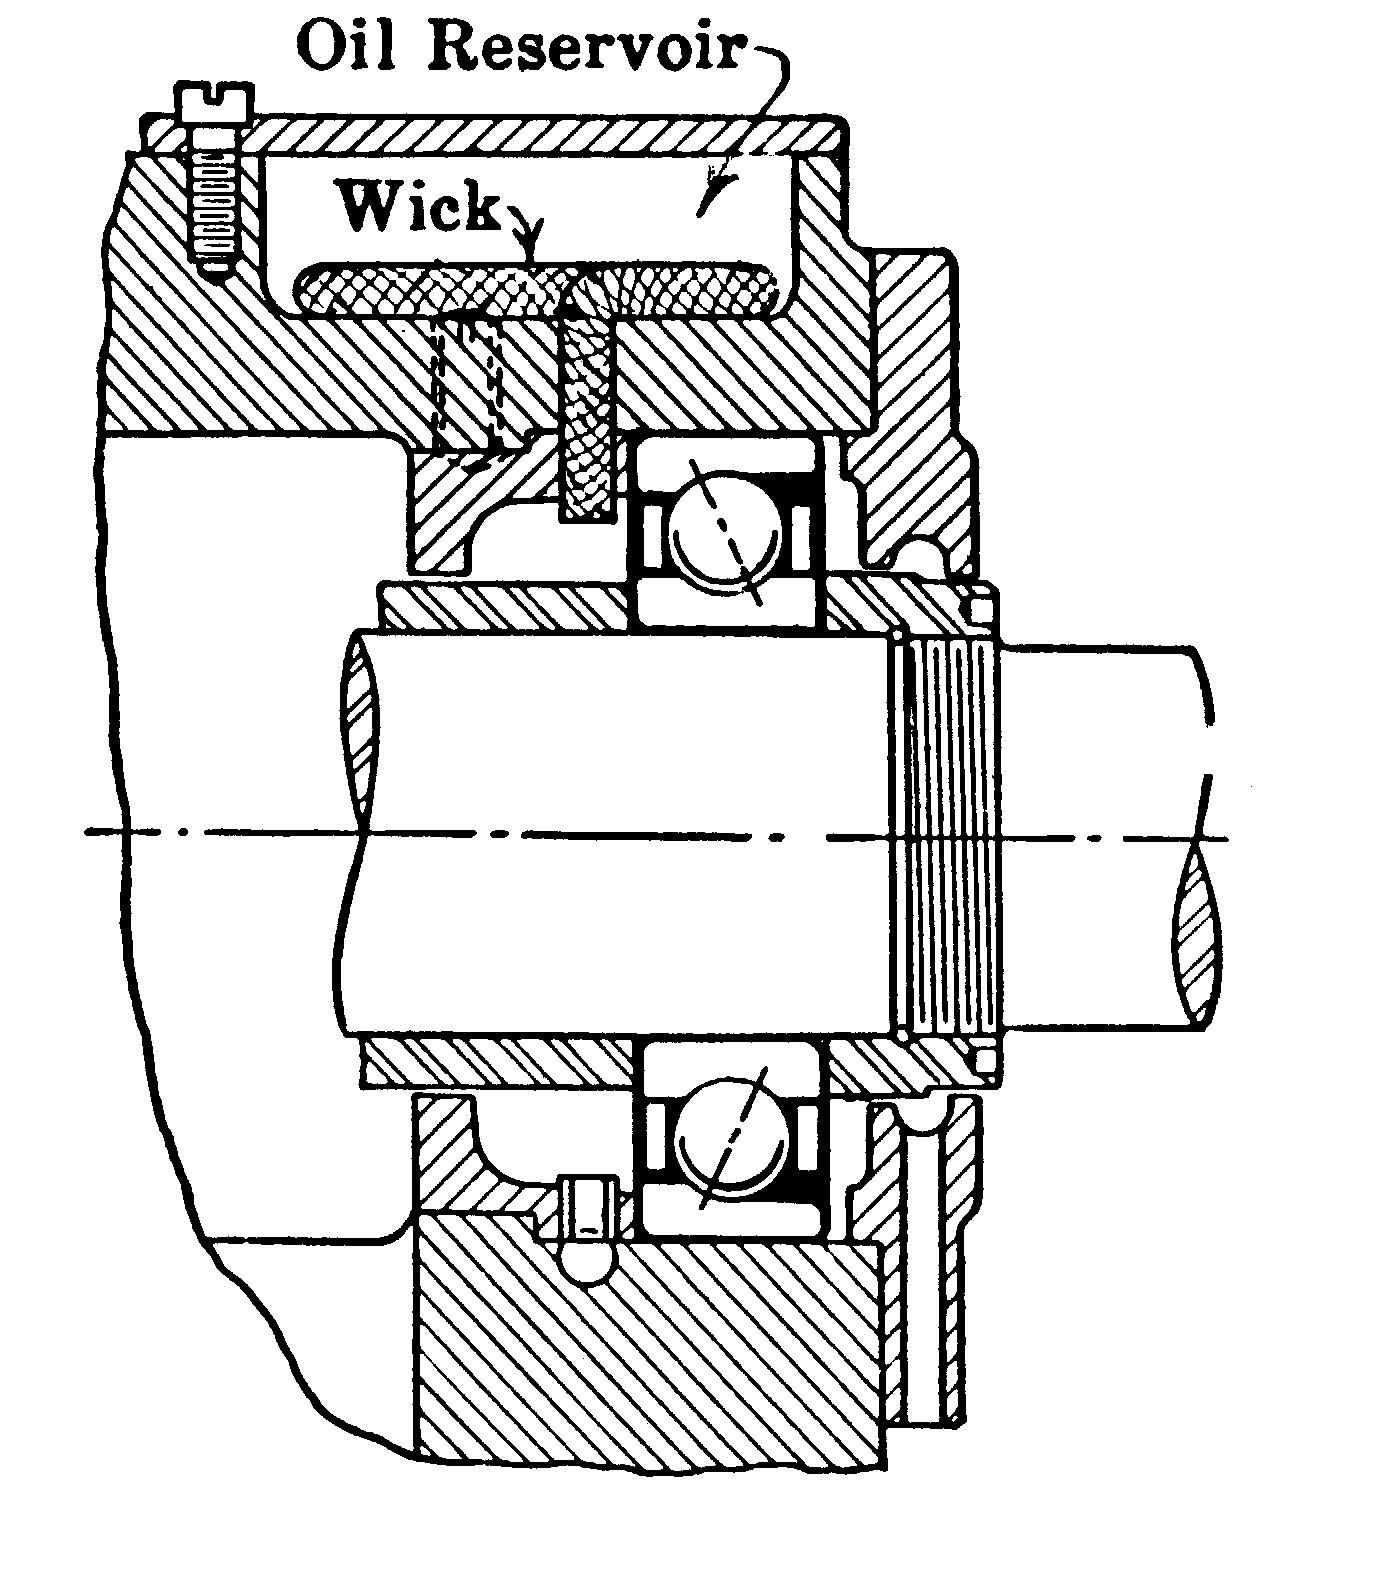
\includegraphics[width=.45\textwidth]{ball-bearing-2}
		\\
		(c) & (d)
	\end{tabular}
%
	\caption{Diverse Maschinenelemente als Beispiel für eine Abbildung mit
	mehreren Elementen. \emph{Overhang Mounting}~(a), \emph{Straddle
	Mounting}~(b), einreihiges Rollenlager~(c), Schmierung von Rollenlagern~
	(d). Diese Abbildung verwendet eine gewöhnliche Tabelle
	(\texttt{tabular}) mit 2 Spalten und 4 Zeilen (Details finden sich im
	Quelltext). Bildquelle~\cite{Faires1934}.}
	\label{fig:Bearings}
\end{figure}


\section{Tabellen}
\label{sec:tabellen}

Tabellen werden häufig eingesetzt um numerische Zusammenhänge, Testergebnisse
etc.\ in übersichtlicher Form darzustellen. Ein einfaches Beispiel ist
Tab.~\ref{tab:programming-languages}, der \latex-Quelltext dazu findet sich in
Prog.~\ref{prog:programming-languages-source}.

Als Argumente der \texttt{tabular}-Umgebung werden die Ausrichtungen der
einzelnen Spalten angegeben. Die Anzahl der Argumente bestimmt somit die
Anzahl der Spalten. Gültige Werte sind \texttt{l} für linksbündig, \texttt{c}
für zentriert und \texttt{r} für rechtsbündig. Die Spaltenbreite ergibt sich
durch die Länge des Inhalts, ein Zeilenumbruch erfolgt nicht. Um die Breite
festzulegen und somit einen Umbruch zu erzeugen, wird \verb|p{Breite}|
verwendet. \texttt{Breite} ist dabei eine gültige Längenangabe, eine
Übersicht über alle gültigen Werte bietet \cite{WikibooksLaTeXLengths2018}.
Die Angabe von \verb|@{}| entfernt den (meist überflüssigen) Rand an den
Seiten der Tabelle.

\begin{table}
	\caption{Programmiersprachen im Überblick.}
	\label{tab:programming-languages}
	\centering
	\setlength{\tabcolsep}{10pt} % separator between columns (standard = 6pt)
	\def\arraystretch{1.25}      % vertical stretch factor (standard = 1.0)
	\begin{tabular}{@{}llll@{}}
		\toprule
		Sprache    & Typ           & Anwendung        & Standardisierung   \\
		\midrule
		C++        & Kompiliert    & Applikationen    & ISO/IEC 14882:2020 \\
		COBOL      & Kompiliert    & Business         & ISO/IEC 1989:2014  \\
		JavaScript & Interpretiert & Web              & ECMA-262           \\
		Python     & Interpretiert & Machine Learning & PEPs               \\
		\bottomrule
	\end{tabular}
\end{table}

\begin{program}
% place caption consistently either at the top or bottom:
	\caption{\latex\ Quelltext zu Tab.~\ref{tab:programming-languages}.
	Die Erzeugung des dargestellten Listings selbst ist in Abschn.\
	\ref{sec:programmtexte} beschrieben.}
	\label{prog:programming-languages-source}
%
\begin{LaTeXCode}[numbers=none]
\begin{table}
	\caption{Programmiersprachen im Überblick.}
	\label{tab:programming-languages}
	\centering
	\setlength{\tabcolsep}{10pt} % separator between columns (standard = 6pt)
	\def\arraystretch{1.25}      % vertical stretch factor (standard = 1.0)
	\begin{tabular}{@{}llll@{}}
		\toprule
		Sprache    & Typ           & Anwendung        & Standardisierung   \\
		\midrule
		C++        & Kompiliert    & Applikationen    & ISO/IEC 14882:2020 \\
		COBOL      & Kompiliert    & Business         & ISO/IEC 1989:2014  \\
		JavaScript & Interpretiert & Web              & ECMA-262           \\
		Python     & Interpretiert & Machine Learning & PEPs               \\
		\bottomrule
	\end{tabular}
\end{table}
\end{LaTeXCode}
%
\end{program}

Der Anspruch an ein ansehnliches Erscheinungsbild von Tabellen ist in den
letzten Jahren zusehends gestiegen. So folgen mittlerweile viele Autor*innen
und auch Verlage, die auf \latex setzen, einigen einfachen
Gestaltungsrichtlinien für Tabellen \cite{Fear2020}, von denen vor allem die
ersten zwei das grundsätzliche Layout der Tabelle bestimmen:

\begin{enumerate}
	\item Nie vertikale Linien benutzen.
	\item Nie doppelte Linien benutzen.
	\item Einheiten in den Spaltenkopf (nicht in den Inhaltsbereich der
	Tabelle) setzen.
	\item Einem Dezimaltrennzeichen geht stets eine Ziffer voran; also $0{,}1$
	nicht bloß ${,}1$.
\end{enumerate}

Das \latex-Paket \texttt{booktabs} ermöglicht es auf einfache Art und Weise,
diesen Anforderungen gerecht zu werden. Innerhalb der
\texttt{tabular}-Umgebung (welche die eigentliche Tabelle definiert) werden
zunächst die Anzahl der Spalten -- bevorzugt linksbündig (\texttt{l}-Angaben)
gesetzt -- definiert. \verb|\toprule| markiert den Beginn der Tabelle, es
folgt die Kopfzeile, die durch \verb|\midrule| abgeschlossen wird. Danach
folgen die Zeilen mit dem Tabelleninhalt. Mittels \verb|\bottomrule| wird die
Tabelle mit einer weiteren horizontalen Linie abgeschlossen.
\verb|\midrule|-Aufrufe können auch öfters vorkommen, um die Tabelle zu
gliedern. Werden horizontale Linien benötigt, die nicht alle Spalten umfassen
sollen, kann \verb|\cmidrule| verwendet werden.

\subsection{Lange Texte in Spalten}

Manchmal ist es notwendig, in Tabellen relativ viel Text in engen Spalten
unter zu bringen, wie in Tab.~\ref{tab:synthesis-techniques}. In diesem Fall
ist es sinnvoll, auf den Blocksatz zu verzichten und gleichzeitig die
strengen Abteilungsregeln zu lockern. Details dazu finden sich im zugehörigen
\latex-Quelltext.


%--------------------------------------------------------------------------------
% Table with narrow columns
%--------------------------------------------------------------------------------
\begin{table}
	\caption{Beispiel für eine Tabelle mit mehrzeiligem Text in engen Spalten.
	Hier werden die Zeilen für den Blocksatz zu kurz, daher wird linksbündig
	gesetzt (im "Flattersatz").}
	\label{tab:synthesis-techniques}
	\centering
	\def\rr{\rightskip=0pt plus1em \spaceskip=.3333em \xspaceskip=.5em\relax}
	\def\arraystretch{1.20}
	\small
	\begin{english}
		\begin{tabular}{@{}p{0.2\textwidth}lp{0.3\textwidth}p{0.2\textwidth}@{}}
			\toprule
			Method & Implem. & Features & Status \\
			\midrule
			{\rr polygon shading} &
			SW/HW &
			{\rr flat-shaded polygons} &
			\\
			{\rr flat shading with z-buffer} &
			SW/HW &
			{\rr depth values} &
			\\
			{\rr goraud shading with z-buffer} &
			SW/HW &
			{\rr smooth shading, simple fog, point light sources} &
			{\rr SGI entry models} \\
			{\rr phong shading with z-buffer} &
			SW/HW &
			{\rr highlights} &
			\\
			{\rr texture mapping with z-buffer} &
			SW/HW &
			{\rr surface textures, simple shadows} &
			{\rr SGI high end, flight simulators} \\
			\bottomrule
		\end{tabular}
	\end{english}
\end{table}

\subsection{Mehrseitige Tabellen}

Oftmals benötigen tabellarische Informationen mehr als nur eine Seite. Hier
wird dann das durch die \texttt{table}-Umgebung erzeugte Floating zum
Problem, denn es verhindert Umbrüche über mehrere Seiten. Um einen
Seitenumbruch in Tabellen zu ermöglichen, kann das \texttt{longtable}-Paket
verwendet werden. Es ersetzt die \texttt{tabular}-Umgebung und benötigt kein
umgebendes \texttt{table}-Environment.

Die Tabelle wird dabei weitgehend gleich definiert, wie in Programm
\ref{prog:programming-languages-source} gezeigt. Hinzu kommen lediglich die
Befehle \verb|\endhead| und \verb|\endfoot|. Sie begrenzen den Kopf- \bzw\
Fußbereich, der auf jeder Seite wiederholt werden soll. Soll dieser für den
Kopfbereich auf der ersten Seite \bzw\ für den Fußbereich auf der letzten
Seite anders sein, können \verb|\endfirsthead| und \verb|\endlastfoot|
verwendet werden.

\texttt{longtable} bietet ebenfalls eine \verb|\caption|-Anweisung, die
jedoch Teil der Tabelle ist und daher mit \verb|\\| abgeschlossen werden muss.
\verb|\label| kann ebenfalls verwendet werden, um auf die Tabelle zu
referenzieren. Dieses sollte jedoch nicht im wiederholenden Kopfbereich
geschehen, da es sonst mehrfach definiert wird. Eine Platzierung im Körper
der Tabelle oder einem mit \verb|\firsthead| definierten Kopfbereich umgeht
dieses Problem.

Tabelle \ref{tab:longtable} zeigt ein Beispiel für eine lange Tabelle. Sollen
horizontale und vertikale Abstände vergrößert werden, müssen diese
Anweisungen vor dem Beginn der Tabelle stehen und mit \verb|{ }| umschlossen
werden.

{\setlength{\tabcolsep}{10pt} % separator between columns (standard = 6pt)
\def\arraystretch{1.50}      % vertical stretch factor (standard = 1.0)
\begin{longtable}{@{}lp{0.23\textwidth}@{}}
	\caption{Eine lange Tabelle, die ggfs.\ über zwei Seiten umbricht.} \\
	\toprule
	Erste Spalte & Zweite Spalte \\
	\midrule\endhead
	\label{tab:longtable}
	Die Spalte rechts enthält viel Text. &
	In dieser Spalte steht viel Text, der eine lange Spalte
	erzeugt. Auch hier kann es Sinn machen, den Inhalt im Flattersatz zu
	setzen. \texttt{longtable} bricht in solchen Spalten jedoch nicht um,
	nur zwischen einzelnen Zeilen. \\
	Hier folgen weitere Zeilen. & Dieser Inhalt dient nur als Platzhalter. \\
	Hier folgen weitere Zeilen. & Dieser Inhalt dient nur als Platzhalter. \\
	Hier folgen weitere Zeilen. & Dieser Inhalt dient nur als Platzhalter. \\
	Hier folgen weitere Zeilen. & Dieser Inhalt dient nur als Platzhalter. \\
	Hier folgen weitere Zeilen. & Dieser Inhalt dient nur als Platzhalter. \\
	Hier folgen weitere Zeilen. & Dieser Inhalt dient nur als Platzhalter. \\
	Hier folgen weitere Zeilen. & Dieser Inhalt dient nur als Platzhalter. \\
	Hier folgen weitere Zeilen. & Dieser Inhalt dient nur als Platzhalter. \\
	Hier folgen weitere Zeilen. & Dieser Inhalt dient nur als Platzhalter. \\
	\bottomrule
\end{longtable}}

\subsection{Spalten und Zeilen verbinden}

Um in einer Tabelle mehrere Spalten zu einer zusammenzufassen wird die Anweisung
%
\begin{quote}
	\verb!\multicolumn{Anzahl}{Format}{Text}!
\end{quote}
%
verwendet. \texttt{Anzahl} definiert die Menge an Spalten, die verbunden
werden sollen. \texttt{Format} gibt die zu verwendende Ausrichtung analog zur
Angabe in \texttt{tabular}-Umgebung an und \texttt{Text} ist der enthaltene
Text.

Um mehrere Zeilen zu einer zusammenzufassen, kann mit
%
\begin{quote}
	\verb!\multirow{Anzahl}{Breite}{Text}!.
\end{quote}
%
eine ähnliche Anweisung verwendet werden. \texttt{Anzahl} repräsentiert hier
die Anzahl an Zeilen, die zu einer verbunden werden sollen. Mit
\texttt{Breite} wird eine Breitenangabe gesetzt. Dabei kommen dieselben
Angaben wie in der \texttt{tabular}-Umgebung zum Einsatz. Zusätzlich können
\texttt{*} und \texttt{=} angegeben werden. Ersteres setzt die durch den Text
entstehende Breite, zweiteres übernimmt die Breite der Spalte aus der
\texttt{tabular}-Angabe. \texttt{Text} ist der zu setzende Inhalt.

Der \verb|multirow|-Befehl wird in der ersten der zu verbindenden Zeilen
gesetzt. Die nachfolgenden Zeilen bleiben leer. Tabelle
\ref{tab:multi-column-row-tabelle} zeigt ein einfaches Beispiel mit
verbundenen Spalten und Zeilen.

\begin{table}
	\caption{Eine Tabelle mit verbundenen Spalten und Zeilen.}
	\label{tab:multi-column-row-tabelle}
	\centering
	\setlength{\tabcolsep}{10pt} % separator between columns (standard = 6pt)
	\def\arraystretch{1.25}      % vertical stretch factor (standard = 1.0)
	\begin{tabular}{@{}lll@{}}
		\toprule
		Spalte 1 & \multicolumn{2}{c}{Spalte 2--3} \\
		\midrule
		Zeile 1  & 
		\multirow{2}{4cm}{Dieser Text erstreckt sich über zwei Zeilen.} &
		\multirow{2}{*}{Dieser Text auch.} \\
	    Zeile 2  & & \\
		\bottomrule
	\end{tabular}
\end{table}


\section{Programmtexte}
\label{sec:programmtexte}

Die Einbindung von Programmtexten (source code) ist eine häufige Notwendigkeit,
\va natürlich bei Arbeiten im Bereich der Informatik.


\subsection{Formatierung von Programmcode}
\label{sec:FormatierungVonProgrammcode}

Es existieren für \latex\ spezielle Pakete zur Darstellung von Programmen,
die \ua\ auch die automatische Nummerierung der Zeilen vornehmen,
insbesondere die Pakete \texttt{listings}%
\footnote{\url{https://ctan.org/pkg/listings}}
und \texttt{listingsutf8}.%
\footnote{\url{https://ctan.org/pkg/listingsutf8}}
Damit sind auch die in Tabelle~\ref{tab:CodeUmgebungen} aufgelisteten
Code-Umgebungen realisiert.
%
\begin{table}
\caption{In \nolinkurl{hgb.sty} vordefinierte Code-Umgebungen.}
\label{tab:CodeUmgebungen}
\centering
\begin{tabular}{@{}lll@{}}
	\toprule
	C (ANSI):    & \verb!\begin{CCode}!
		& \verb!...! \verb!\end{CCode}! \\
	C++ (ISO):   & \verb!\begin{CppCode}!
		& \verb!...! \verb!\end{CppCode}! \\
	C\#:         & \verb!\begin{CsCode}!
		& \verb!...! \verb!\end{CsCode}! \\
	CSS:         & \verb!\begin{CssCode}!
		& \verb!...! \verb!\end{CssCode}! \\
	HTML:        & \verb!\begin{HtmlCode}!
		& \verb!...! \verb!\end{HtmlCode}! \\
	Java:        & \verb!\begin{JavaCode}!
		& \verb!...! \verb!\end{JavaCode}! \\
	JavaScript:  & \verb!\begin{JsCode}!
		& \verb!...! \verb!\end{JsCode}! \\
	\latex:      & \verb!\begin{LaTeXCode}!
		& \verb!...! \verb!\end{LaTeXCode}! \\
	Objective-C: & \verb!\begin{ObjCCode}!
		& \verb!...! \verb!\end{ObjCCode}! \\
	PHP:         & \verb!\begin{PhpCode}!
		& \verb!...! \verb!\end{PhpCode}! \\
	Python:      & \verb!\begin{PythonCode}!
		& \verb!...! \verb!\end{PythonCode}! \\
	Swift:       & \verb!\begin{SwiftCode}!
		& \verb!...! \verb!\end{SwiftCode}! \\
	XML:         & \verb!\begin{XmlCode}!
		& \verb!...! \verb!\end{XmlCode}! \\
	Generisch:   & \verb!\begin{GenericCode}!
		& \verb!...! \verb!\end{GenericCode}! \\
	\bottomrule
\end{tabular}
\end{table}
%
Die Verwendung ist äußerst einfach, \zB\ für Quellcode in der
Programmiersprache C schreibt man
%
\begin{quote}
\begin{verbatim}
\begin{CCode}
    ... 
\end{CCode}
\end{verbatim}
\end{quote}
%
Der Quellcode innerhalb dieser Umgebungen wird in der jeweiligen
Programmiersprache interpretiert, wobei Kommentare erhalten bleiben. Diese
Umgebungen können sowohl alleinstehend (im Fließtext) oder innerhalb von
Float-Umgebungen (insbes.\ \texttt{program}) verwendet werden. Im ersten Fall
wird der Quelltext auch über Seitengrenzen umgebrochen. Mit \verb!/+! ...
\verb!+/! ist eine Escape-Möglichkeit nach \latex\ vorgesehen, die \va\ zum
Setzen von Labels für Verweise auf einzelne Programmzeilen nützlich ist, \zB\
mit
%
\begin{quote}
	\verb!/+\label{ExampleCodeLabel}+/!
\end{quote}
%
Ein Beispiel mit Java ist in Prog.~\ref{prog:CodeExample} gezeigt, wobei der
oben angeführte Label in Zeile \ref{ExampleCodeLabel} steht. Man beachte,
dass innerhalb der Kommentare auch mathematischer Text (wie etwa in Zeile
\ref{MathInCode} von Prog.~\ref{prog:CodeExample}) stehen kann.


\subsubsection{Nummerierung der Code-Zeilen}

Alle in Tabelle~\ref{tab:CodeUmgebungen} angeführten Code-Umgebungen können
mit optionalen Argumenten verwendet werden, die insbesondere zur Steuerung
der Zeilennummerierung hilfreich. Im Normalfall (also ohne zusätzliche
Angabe) mit
%
\begin{quote}
	\verb!\begin{!\texttt{\emph{some}Code}\verb!} ... !
\end{quote}
%
werden alle Code-Zeilen (einschließlich der Leerzeilen) bei 1 beginnend und
fortlaufend nummeriert. Bei aufeinanderfolgenden Codesegmenten ist es oft
hilfreich, die Nummerierung aus dem vorherigen Abschnitt kontinuierlich
weiter laufen zu lassen, ermöglicht durch die Angabe des optionalen Arguments
\texttt{firstnumber={\obnh}last}:
%
\begin{quote}
	\verb!\begin{!\texttt{\emph{some}Code}\verb!}[firstnumber=last] ... !
\end{quote}
%
Um die Nummerierung der Codezeilen gänzlich zu unterbinden genügt die Angabe
des optionalen Arguments \texttt{numbers={\obnh}none}:
%
\begin{quote}
	\verb!\begin{!\texttt{\emph{some}Code}\verb!}[numbers=none] ... !
\end{quote}
%
In diesem Fall ist natürlich die Verwendung von Zeilenlabels im Code nicht
sinnvoll.


\subsection{Platzierung von Programmcode}

Da Quelltexte sehr umfangreich werden können, ist diese Aufgabe nicht immer
leicht zu lösen. Abhängig vom Umfang und vom Bezug zum Haupttext gibt es
grundsätzlich drei Möglichkeiten zur Einbindung von Programmtext:
%
\begin{itemize}
	\item[a)] im laufenden Text für kurze Programmstücke,
	\item[b)] als Float-Element (\texttt{program}) für mittlere Programmtexte
	bis max.\ eine Seite oder
	\item[c)] im Anhang (für lange Programmtexte).
\end{itemize}

\subsubsection{Programmtext im laufenden Text}

Kurze Codesequenzen können ohne weiteres im laufenden Text eingebettet
werden, sofern sie an den gegebenen Stellen von unmittelbarer Bedeutung sind.
Die folgende (rudimentäre) Java-Methode \texttt{extractEmail} sucht nach
einer E-Mail-Adresse in der Zeichenkette \texttt{line}:
%
\begin{JavaCode}[numbers=none]
static String extractEmail(String line) {
    line = line.trim(); // find the first blank
    int i = line.indexOf(' '); 
    if (i > 0)
        return line.substring(i).trim();
    else
        return null;
}
\end{JavaCode}
%
\noindent
Dieses Codestück wurde mit 
%
\begin{quote}
\begin{verbatim}
\begin{JavaCode}[numbers=none]
static String extractEmail(String line) {
    line = line.trim(); // find the first blank
    ...
}
\end{JavaCode}
\end{verbatim}
\end{quote}
%
erstellt (siehe Abschn.\ \ref{sec:FormatierungVonProgrammcode}). In-line
Programmstücke sollten maximal einige Zeilen lang sein und nach Möglichkeit
nicht durch Seitenumbrüche geteilt werden.


\subsubsection{Programmtexte als Float-Elemente}

Sind längere Codesequenzen notwendig, die in unmittelbarer Nähe des laufenden
Texts stehen müssen, sollten diese genauso wie andere Abbildungen als
Float-Elemente behandelt werden. Diese Programmtexte sollten den Umfang von
einer Seite nicht übersteigen. Im Notfall können auch bis zu zwei Seiten in
aufeinanderfolgende Abbildungen gepackt werden, jeweils mit eigener Caption.
In \texttt{hgb.sty} ist eine neue Float-Umgebung \texttt{program} definiert,
die analog zu \texttt{table} verwendet wird:
%
\begin{quote}
\begin{verbatim}
\begin{program}
\caption{Der Titel zu diesem Programmstück.}
\label{prog:xyz}
\begin{JavaCode}
  class Foo {
    ...
  }
\end{JavaCode}
\end{program}
\end{verbatim}
\end{quote}
%
Wenn gewünscht, kann die Caption auch unten angebracht werden (jedenfalls
aber konsistent und nicht gemischt). Natürlich darf auch hier nicht mit einer
linearen Abfolge im fertigen Druckbild gerechnet werden, daher sind Wendungen
wie "\ldots\ im folgenden Programmstück \ldots" zu vermeiden und
entsprechende Verweise einzusetzen. Beispiele sind die Programme
\ref{prog:programming-languages-source} und \ref{prog:CodeExample}.

\begin{program}
% place caption consistently either at the top or bottom:
\caption{Beispiel für die Auflistung von (Java) Programmcode als Float-Element.}
\label{prog:CodeExample}
\begin{JavaCode}
import ij.ImagePlus;
import ij.plugin.filter.PlugInFilter;
import ij.process.ImageProcessor;

public class My_Inverter implements PlugInFilter {
	int agent_velocity;
	String title = ""; 				// just to test printing of double quotes

	public int setup (String arg, ImagePlus im) {
		return DOES_8G;
	}

	public void run (ImageProcessor ip) {
		int w = ip.getWidth(); /+\label{ExampleCodeLabel}+/
		int h = ip.getHeight();

		/* iterate over all image coordinates */
		for (int u = 0; u < w; u++) {
			for (int v = 0; v < h; v++) {
				int p = ip.getPixel(u, v);
				ip.putPixel(u, v, 255 - p); // invert: /+\smash{$I'(u,v) \leftarrow (255 - I(u,v))$}\label{MathInCode}+/
			}
		}
	}
} // end of class /+My\_Inverter+/
\end{JavaCode}
%
\end{program}


\subsubsection{Programmtext im Anhang}

Für längere Programmtexte, speziell wenn sie vollständige Implementierungen
umfassen und im aktuellen Kontext nicht unmittelbar relevant sind, muss zur
Ablage in einem getrennten Anhang am Ende des Dokuments gegriffen werden. Für
Hinweise auf bestimmte Details können entweder kurze Ausschnitte in den
laufenden Text gestellt oder mit entsprechenden Seitenverweisen gearbeitet
werden. Ein solches Beispiel ist der \latex-Quellcode in Anhang
\ref{app:latex} (Seite \pageref{app:latex}).%
\footnote{Grundsätzlich ist zu überlegen, ob die gedruckte Einbindung der
gesamten Programmtexte einer Implementierung für den*die Leser*in überhaupt
sinnvoll ist, oder ob diese nicht besser elektronisch (auf Datenträger)
beigefügt und nur exemplarisch beschrieben werden.}
